% Gemini theme
% See: https://rev.cs.uchicago.edu/k4rtik/gemini-uccs
% A fork of https://github.com/anishathalye/gemini

\documentclass[final]{beamer}

% ====================
% Packages
% ====================
\usepackage{amsfonts}
\usepackage[T1]{fontenc}
\usepackage{lmodern}
\usepackage[size=custom,width=120,height=72,scale=1.0]{beamerposter}
\geometry{paperwidth=48in,paperheight=36in}
\usetheme{gemini}
\usecolortheme{ucf}
\usepackage{graphicx}
\usepackage{booktabs}
\usepackage{tikz}
\usepackage{pgfplots}
\pgfplotsset{compat=1.14}

\usepackage{float}
\usepackage{xspace}
\usepackage{graphicx}
\graphicspath{{./imgs/}}
\usepackage{comment}
\usepackage{listings,hyperref}
\usepackage{cite}
\usepackage{hyperref}

% nice looking audit titles
\newcommand{\Minerva}{\textsc{Minerva}\xspace}
\newcommand{\Prov}{\textsc{Providence}\xspace}
\newcommand{\B}{{{B2}}\xspace}
\newcommand{\R}{{{R2}}\xspace}
\newcommand{\BRAVO}{\textsc{BRAVO}\xspace}


% ====================
% Lengths
% ====================

% If you have N columns, choose \sepwidth and \colwidth such that
% (N+1)*\sepwidth + N*\colwidth = \paperwidth
\newlength{\sepwidth}
\newlength{\colwidth}
\setlength{\sepwidth}{0.001\paperwidth}
\setlength{\colwidth}{0.23\paperwidth}

\newcommand{\separatorcolumn}{\begin{column}{\sepwidth}\end{column}}

% ====================
% Title
% ====================

\title{Election Security with Risk-Limiting Audits}

%\author{Nitish A. Gupta \inst{1} \and Nitish A. Gupta \inst{2}}
\author{Oliver Broadrick\inst{1} \and
Poorvi L. Vora\inst{1} \and
Filip Zag{\'o}rski\inst{2}\inst{3}}
% First names are abbreviated in the running head.
% If there are more than two authors, 'et al.' is used.
%
\institute[shortinst]{\inst{1} Department of Computer Science, The George Washington University%\thanks{Supported in part by NSF Award 2015253} 
\samelineand \inst{2} Wroclaw University of Science and Technology%\thanks{Author was partially supported by Polish National Science Centre contract number DEC-2013/09/D/ST6/03927} and 
\samelineand \inst{3} Votifica
}
%

%\institute[shortinst]{\inst{1} \textit{University of Central Florida, Orlando, FL} \samelineand \inst{2} Another Institute}

% ====================
% Footer (optional)
% ====================

\footercontent{
  \href{odbroadrick@gmail.com}{odbroadrick@gmail.com}
}
% (can be left out to remove footer)

% ====================
% Logo (optional)
% ====================

% use this to include logos on the left and/or right side of the header:
% \logoright{\includegraphics[height=7cm]{logo1.pdf}}
% \logoleft{\includegraphics[height=7cm]{logo2.pdf}}

% ====================
% Body
% ====================

\begin{document}
\addtobeamertemplate{headline}{}
{
    \begin{tikzpicture}[remember picture,overlay]
      \node [anchor=north west, inner sep=3cm] at ([xshift=0.0cm,yshift=3cm]current page.north west)
      {
\includegraphics[height=8cm]{logos/gw.png}}; % also try shield-white.eps
      \node [anchor=north east, inner sep=3cm] at ([xshift=0.0cm,yshift=3cm]current page.north east)
      {
\includegraphics[height=8cm]{logos/gw.png}};
    \end{tikzpicture}
}

\begin{frame}[t]
\begin{columns}[t]
\separatorcolumn

\begin{column}{\colwidth}

\begin{block}{Original Contributions}

Risk-Limiting Audits (RLAs) are rigorous election audits performed in rounds. 
RLAs EoR \BRAVO and SO \BRAVO \cite{bravo} rely on the Sequential Probability Ratio Test (SPRT), using
a ratio of sample probabilities conditioned on alternative and null hypotheses.
More recent RLA \Minerva \cite{usenix_minerva} uses a ratio of the tails of the same distributions, and requires half as many
ballots as EoR \BRAVO in a first round with probability of stopping $0.9$.
Understanding audit behavior for later rounds has no easy analytical approach.
\Minerva was used in a pilot RLA in Montgomery County, Ohio in 2020,
and is recommended by the largest US voting organizations: Verified Voting, the Brennan Center, and Common Cause.
%It is unknown how the audits compare in later rounds or with lower stopping probabilities, a problem with no easy analytical approach.

\begin{itemize}
\item
We provide simulations \cite{simulations} of EoR \BRAVO, SO \BRAVO, and \Minerva that help us understand their behavior across multiple rounds and with lower
first round stopping probability; this information can be used to advise election officials.
\end{itemize}

Unlike EoR and SO \BRAVO, \Minerva is proven to be risk-limiting only when round sizes are predetermined, 
meaning round sizes cannot be chosen based on previous samples, flexibility that may have meaningful impact on workload.

\begin{itemize}
\item We introduce \Prov, an RLA which has the efficient tail ratio approach of \Minerva but is resistant to an adversary who can pick
future round sizes with knowledge of previous samples. 
\item \Prov was named after the Rhode Island city where it was used for a public
pilot audit in February 2022.
\end{itemize}
\end{block}

\begin{block}{Results}

\begin{itemize}
\item \BRAVO audits are more conservative than \Minerva, which stops with fewer ballots, for both first round stopping probabilities
\item Advantage of using \Minerva decreases considerably for smaller first round stopping probability
\item Proofs that \Prov is risk-limiting and resistant to an adversary who can pick future round sizes with knowledge of previous samples
\end{itemize}
\end{block}

\begin{block}{Risk-Limiting Audits}

\begin{itemize}
\item
A risk-limiting audit (RLA) draws paper ballots in rounds, stopping if a rigorous statistical criterion is satisfied, or proceeding to a full hand count. If the announced outcome of the election is erroneous, an RLA will detect the error with high, predetermined minimum probability. 
\item
An audit $\mathcal{A}$ takes a sample of ballots $X$ as input and gives as output either
(1) $Correct$: the audit is complete, or (2) $Uncertain$: continue the audit.
\item
The maximum risk $R$ of audit $\mathcal{A}$ with sample $X\in \{0,1\}^*$ drawn from 
the true underlying distribution of ballots is
$$R(\mathcal{A})=\Pr[\mathcal{A}(X)=Correct \mid H_0],$$ where $H_0$ is the null
hypothesis: the true underlying election is a tie.
\item
An audit $\mathcal{A}$ is a Risk-Limiting Audit with 
risk limit $\alpha$ iff 
$$R(\mathcal{A}) \le \alpha.$$
\end{itemize}
\end{block}

\begin{block}{Simulations}

\begin{itemize}
\item 
Software: R2B2 library\cite{r2b2} which has Python implementations of several RLAs as well as a simulator
\item 
Risk limit: 10\%
\item
Margins: 2020 US Presidential election statewide results, limiting ourselves to pairwise margins
for the two main candidates of $0.05$ or larger
\item 
Trials per state: $10,000=10^4$ audits assuming the underlying election is as announced,  
and $10,000=10^4$ audits assuming the underlying election is a tie
\item 
Round schedules: EoR \BRAVO and SO \BRAVO round sizes are chosen to achieve the same
probability of stopping in each round given preceding samples. \Minerva first round sizes
are chosen to achieve some probability of stopping and subsequent round sizes are given by multiplying the previous
round size by $1.5$ or by $1.0$.
\end{itemize}
\end{block}

\end{column}

\separatorcolumn

\begin{column}{\colwidth}

\begin{block}{Risk}

\begin{itemize}
\item 
All audits have estimated risks below the risk limit
\item
EoR \BRAVO falls an order of magnitude less than the others, unnecessarily conservative
\end{itemize}

\begin{figure}[h]
\centering
\begin{minipage}{.49\textwidth}
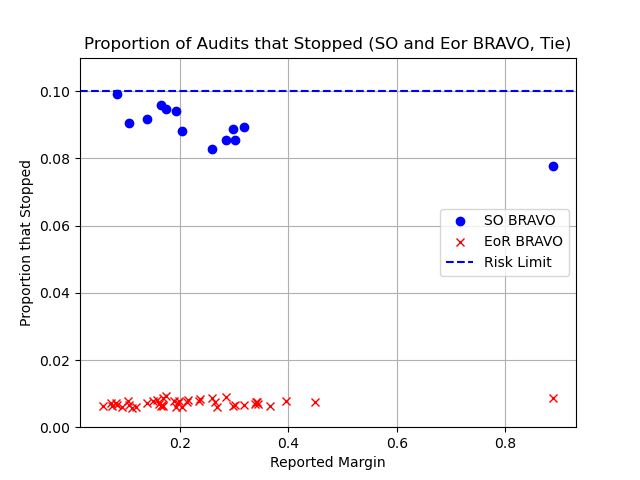
\includegraphics[width=\textwidth]{bravo_risks.png}
\label{fig:bravo_risk}
\end{minipage}
\begin{minipage}{.49\textwidth}
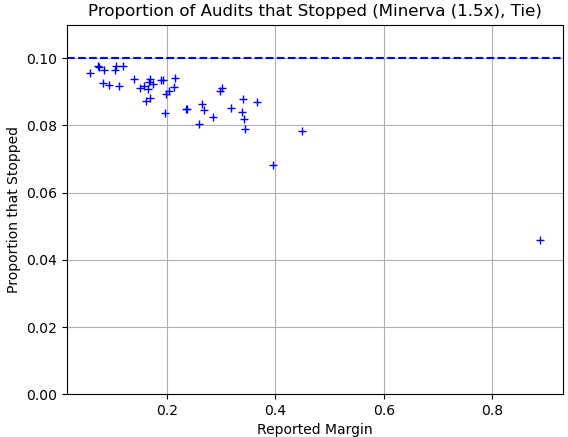
\includegraphics[width=1.0\textwidth]{riskminerva1p5_10t4.png}
\label{fig:minerva_risk}
\end{minipage}
\caption{For $\chi_1=0.9$ the fraction of audits (EoR \BRAVO (left), SO \BRAVO (left), and \Minerva with multiplier $1.5$ (right)) that stopped in any of the $5$ rounds when the underlying election was a tie. (For SO \BRAVO audits we show the 13 states for which simulations are complete.)}
%\label{fig:risk}
\end{figure}

\end{block}


\begin{block}{Stopping Probability}

\begin{itemize}
\item
Conditional stopping probability, $\chi_j$, is the probability that an audit will stop in round $j$ given that it did not stop earlier, and in 
simulations $\chi_j$ is estimated by the proportion of audits that stop in a round to those that ``entered'' that round
i.e. those that did not stop before round $j$. 
%TODO move this more rigorous definition somewhere else
%The conditional stopping probability  of an audit $\mathcal{A}$ in round $j$ is 
%$$\chi_j (\mathcal{A})=\Pr[\mathcal{A}(X)=Correct ~in~round~j~\mid H_a \land \mathcal{A}(X) \neq Correct ~previously]$$
\end{itemize}

\begin{figure}[h]
\centering
\begin{minipage}{.49\textwidth}
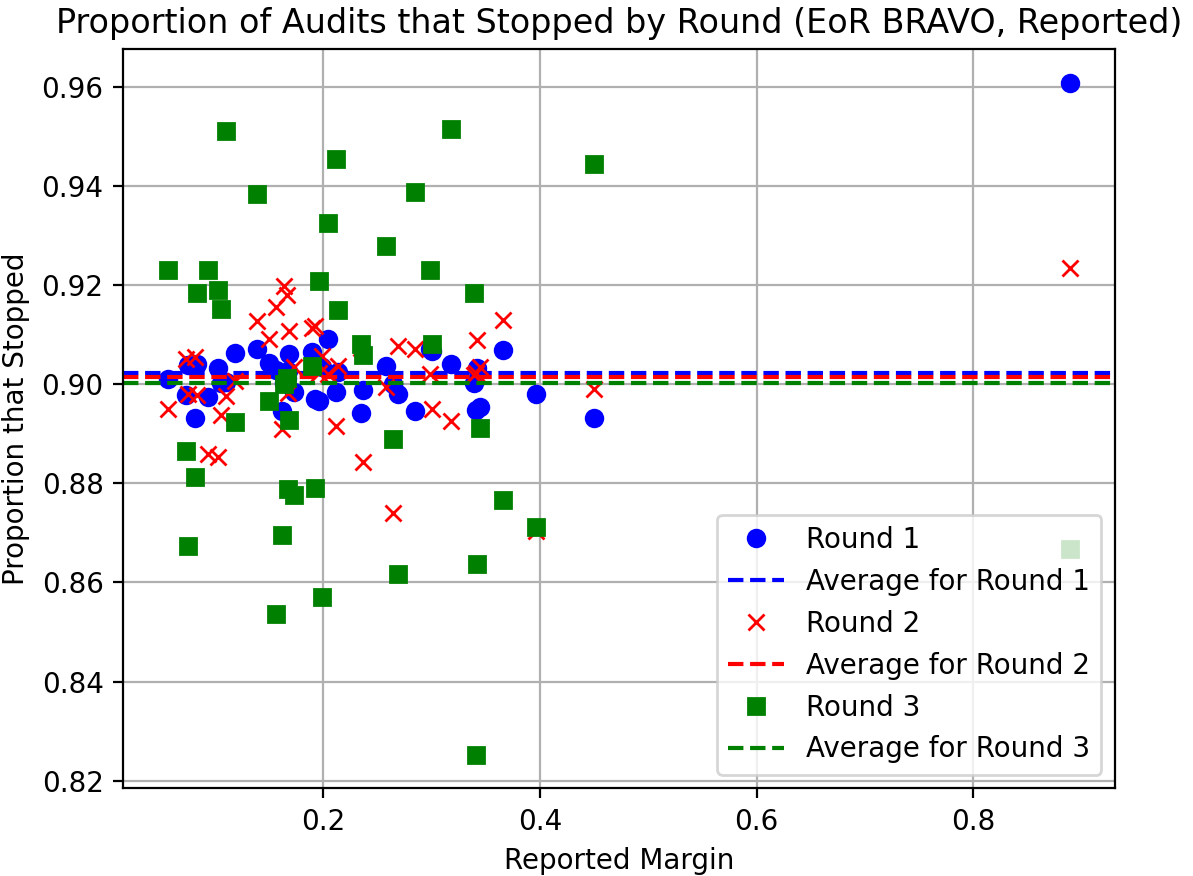
\includegraphics[width=1.0\textwidth]{eor_bravo_90perc_10^4_corrected/sprob_first_three_cropped.png}
\label{fig:eor_bravo_sprob}
\end{minipage}
\begin{minipage}{.49\textwidth}
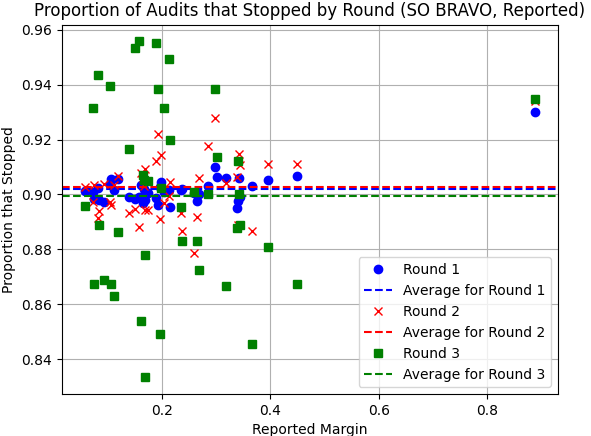
\includegraphics[width=1.0\textwidth]{so_bravo_90perc_10^4/sprob_first_three.png}
\label{fig:so_bravo_sprob}
\end{minipage}
\caption{For each state margin, when the underlying election is as announced, the number of audits that stopped in the $j^{th}$ round, as a fraction of all audits which had not yet stopped before the $j^{th}$ round for $j=1,2,3$ and $\chi_j=0.9$. The left shows EoR \BRAVO and the right shows SO \BRAVO.}
\end{figure}

\begin{figure}[h]
\centering
\begin{minipage}{.49\textwidth}
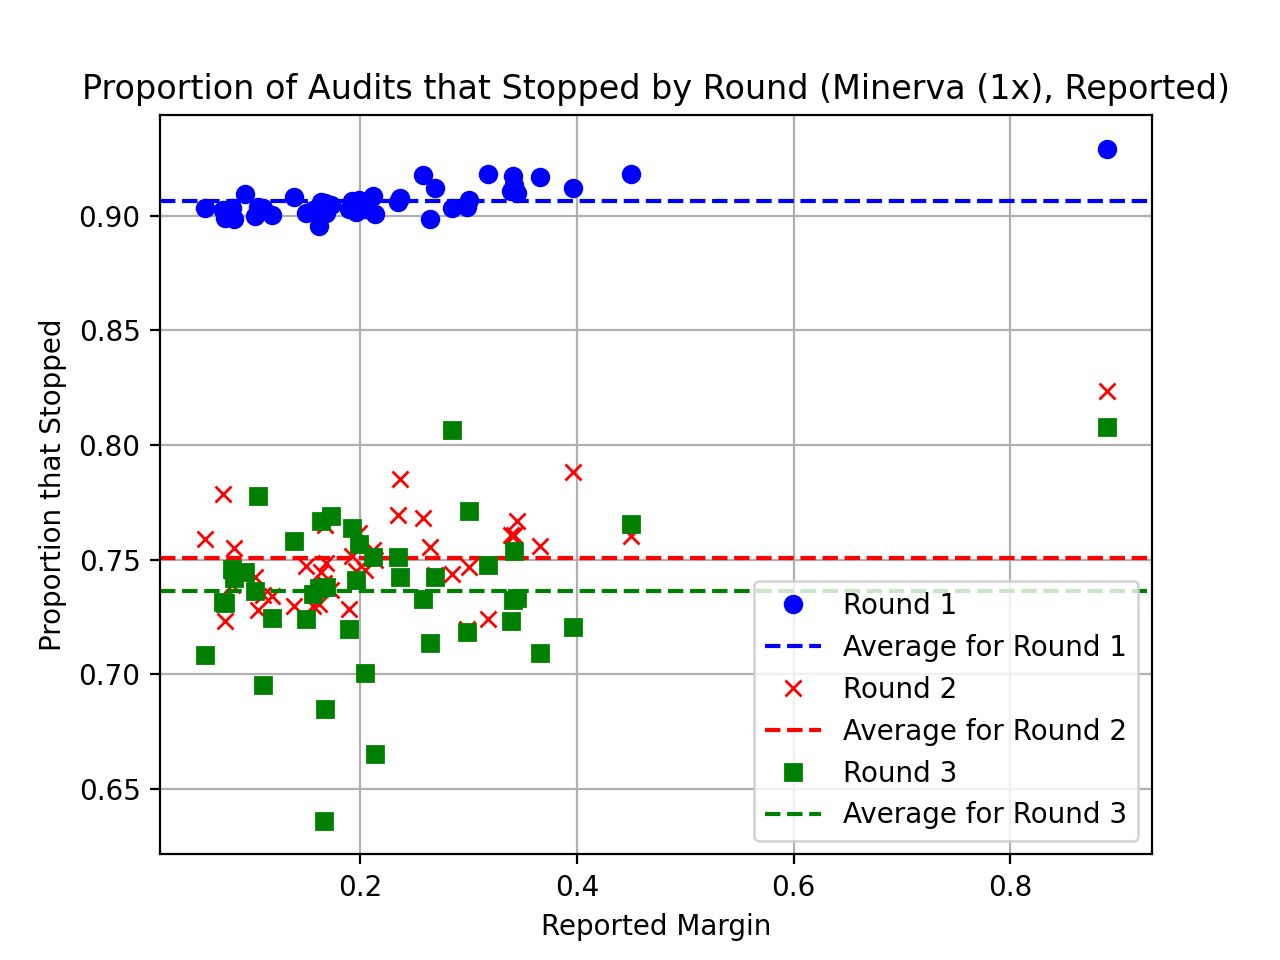
\includegraphics[width=1\textwidth]{minerva_multiround_1x_10^4/sprobs_first_three.png}
\label{fig:minerva1_sprob}
\end{minipage}
\begin{minipage}{.49\textwidth}
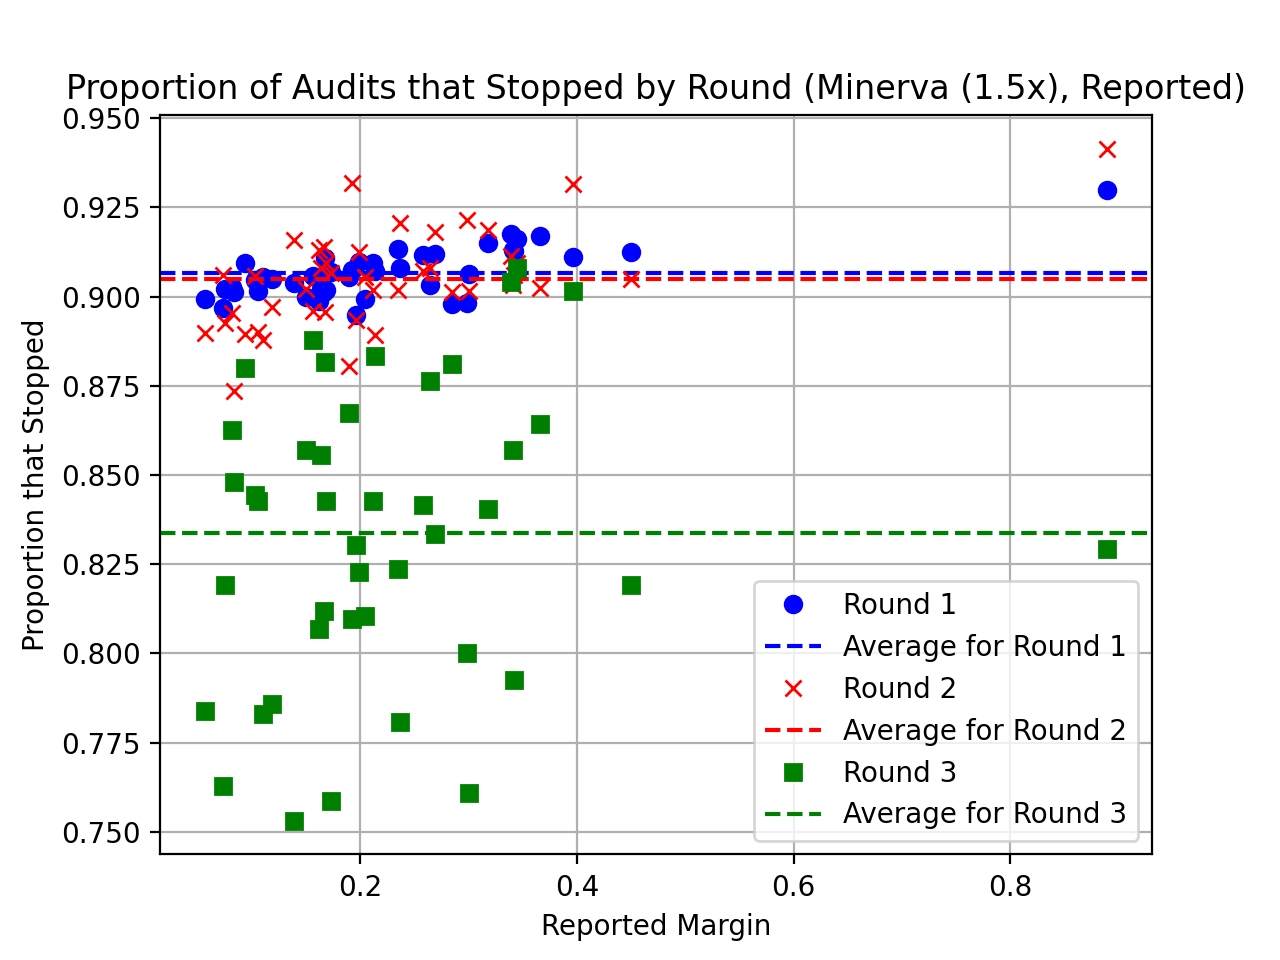
\includegraphics[width=1\textwidth]{minerva_multiround_1p5x_10^4/sprobs_first_three.png}
\label{fig:minerva1p5_sprob}
\end{minipage}
\caption{When the underlying election is as announced, the number of \Minerva audits that stopped in the $j^{th}$ round, as a fraction of all \Minerva audits which had not yet stopped before the $j^{th}$ round for $j=1,2,3$. The left shows \Minerva with the round schedule obtained by $\chi_1=0.9$ and round size multiple $1.5$.}
\end{figure}

\begin{figure}
\begin{centering}
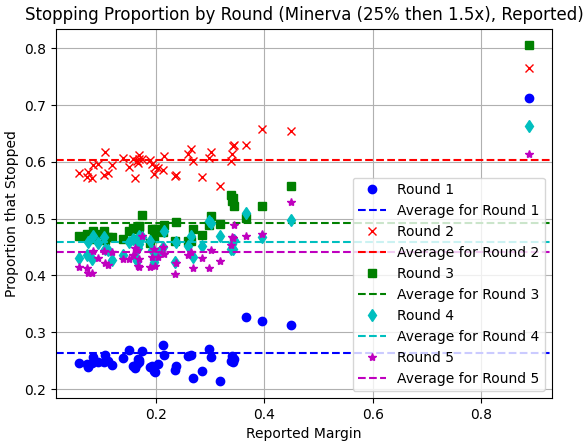
\includegraphics[width=0.5\textwidth]{minerva25percthen1p5_sprob.png}
\caption{For each state margin, when the underlying election is as announced, the number of \Minerva audits that stopped in the $j^{th}$ round,
as a fraction of all \Minerva audits which had not yet stopped before the $j^{th}$ round for $j=1,2,3$, round size multiple of $1.5$ and $\chi_1 = 0.25$.}
\label{fig:minerva_25}
\end{centering}
\end{figure}

\end{block}

\end{column}

\separatorcolumn

\begin{column}{\colwidth}

\begin{block}{Number of Ballots}

\begin{itemize}
\item
The number of ballots sampled is one crude measure of the workload of an audit.
To keep the costs of RLAs low, audits should be designed to stop with as few ballots as possible.
\item
The following plots show the probability of stopping as a function of the average number of ballots
sampled by round in our simulations.
\end{itemize}

\begin{figure}[h]
\centering
\begin{minipage}{.49\textwidth}
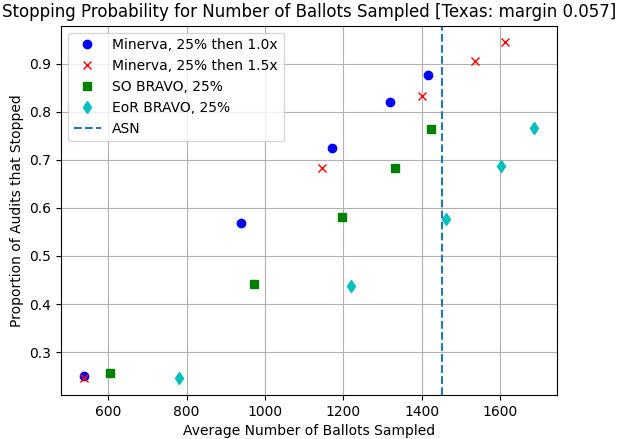
\includegraphics[width=1\textwidth]{texas25.png}
\label{fig:texas_25}
\end{minipage}
\begin{minipage}{.49\textwidth}
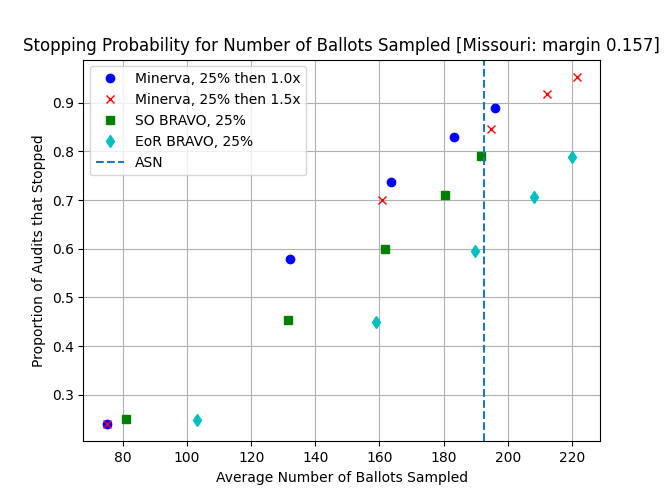
\includegraphics[width=1\textwidth]{missouri25.png}
\label{fig:missouri_25}
\end{minipage}
\caption{Cumulative fraction of audits that stopped as a function of average number of sampled ballots for all four audits we studied, for the states of Texas with margin $.057$ (left) and Missouri with margin $0.157$ (right), both with first round stopping probability $\chi_1=0.25$.}
\end{figure}

\begin{figure}[h]
\centering
\begin{minipage}{.49\textwidth}
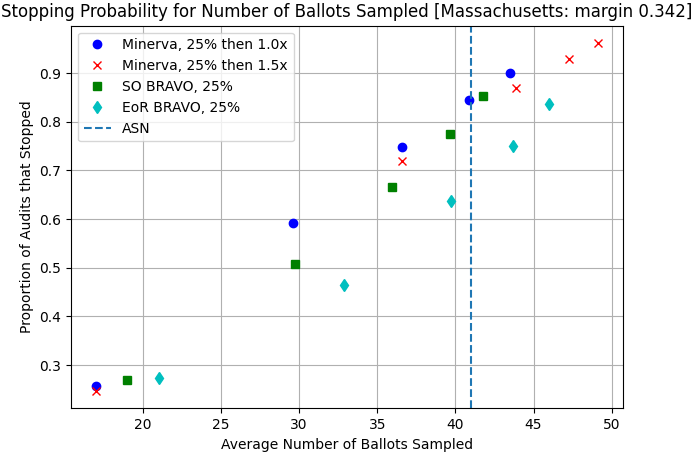
\includegraphics[width=1\textwidth]{massachusetts25.png}
\label{fig:mass_25}
\end{minipage}
\begin{minipage}{.49\textwidth}
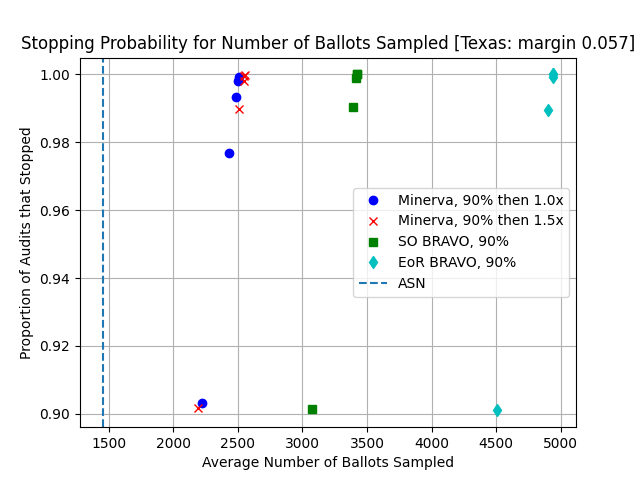
\includegraphics[width=1\textwidth]{texas90.png}
\label{fig:texas_90}
\end{minipage}
\caption{Cumulative fraction of audits that stopped as a function of average number of sampled ballots for all four audits we studied, for the states Massachusetts (left) with margin $0.342$ and $\chi_1=0.25$ and Texas (right) with margin $0.057$ and $\chi_1=0.9$.}
\end{figure}

For $\chi_1=0.25$, the ratio of first round size of EoR \BRAVO to \Minerva is $1.45$, $1.37$, $1.23$ for states Texas, Missouri and Massachusetts, and margins $0.057$, $0.157$ and $0.342$ respectively. This may be compared to $2.03$, $1.99$ and $1.8$ respectively for $\chi_1=0.9$. Similarly, for $\chi_1=0.25$, the ratio of first round size of SO \BRAVO to \Minerva is $1.13$, $1.08$, $1.12$ for states Texas, Missouri and Massachusetts, and margins $0.057$, $0.157$ and $0.342$ respectively. This may be compared to $1.38$, $1.38$ and $1.30$ respectively for $\chi_1=0.9$. 

\end{block}

\begin{block}{Providence}

\begin{itemize}
\item
The efficiency of \Minerva is great, but it lacks the flexibility of \BRAVO in choosing round sizes based on previous samples.
\item
\Prov is our novel RLA which has the efficiency of \Minerva and the flexibility of \BRAVO.
\item For alternative hypothesis $H_a$ that the election is truly as announced and null
hypothesis $H_0$ that the true election is a tie, \BRAVO has the stopping condition that
for $k$ cumulative ballots for the winner and $n$ cumulative sampled ballots,
$$\sigma(k,n,p_a,p_0) \triangleq \frac{\Pr[K=k\mid H_a, n]}{\Pr[K=k\mid H_0, n]}\ge \frac{1}{\alpha}.$$
\item \Minerva has the stopping condition that in round $j$ with cumulative winner ballots $k_j$ and round sizes $\bar n_j = n_1,n_2,\ldots,n_j$
$$\tau_j(k_j,\bar n_j,p_a,p_0) \triangleq \frac{\Pr[K_j\ge k_j \wedge \mathcal{A}_{i<j}(X)\neq Correct \mid H_a, \bar n_j]}{\Pr[K_j\ge k_j \wedge \mathcal{A}_{i<j}(X)\neq Correct \mid H_0, \bar n_j]}\ge \frac{1}{\alpha}.$$ Testing this stopping condition requires computationaly expensive convolutions.
\item The \Prov stopping condition uses ideas from both \BRAVO and \Minerva and requires no convolution to test:
$$\omega_j(k_{j-1},k_j,n_{j-1},n_j,p_a,p_0)\triangleq \sigma(k_{j-1},n_{j-1},p_a,p_0)\cdot \tau_1(k_j,n_j,p_a,p_0) \ge \frac{1}{\alpha}.$$ 
\end{itemize}

\heading {Resistance against an adversary} 
If for each round $j=1,2,\ldots$, 
adversary $\mathcal{A}$ has knowledge of all previous samples 
and is allowed to choose round size $n_{j+1}$ for round $j+1$, 
\Prov is still risk-limiting. 


\end{block}

\end{column}

\separatorcolumn

\begin{column}{\colwidth}

\begin{block}{Providence Pilot}

In February 2022, The Rhode Island Board of Elections hosted a public pilot \Prov RLA which 
passed (met the risk limit) in the first round.

\begin{figure}
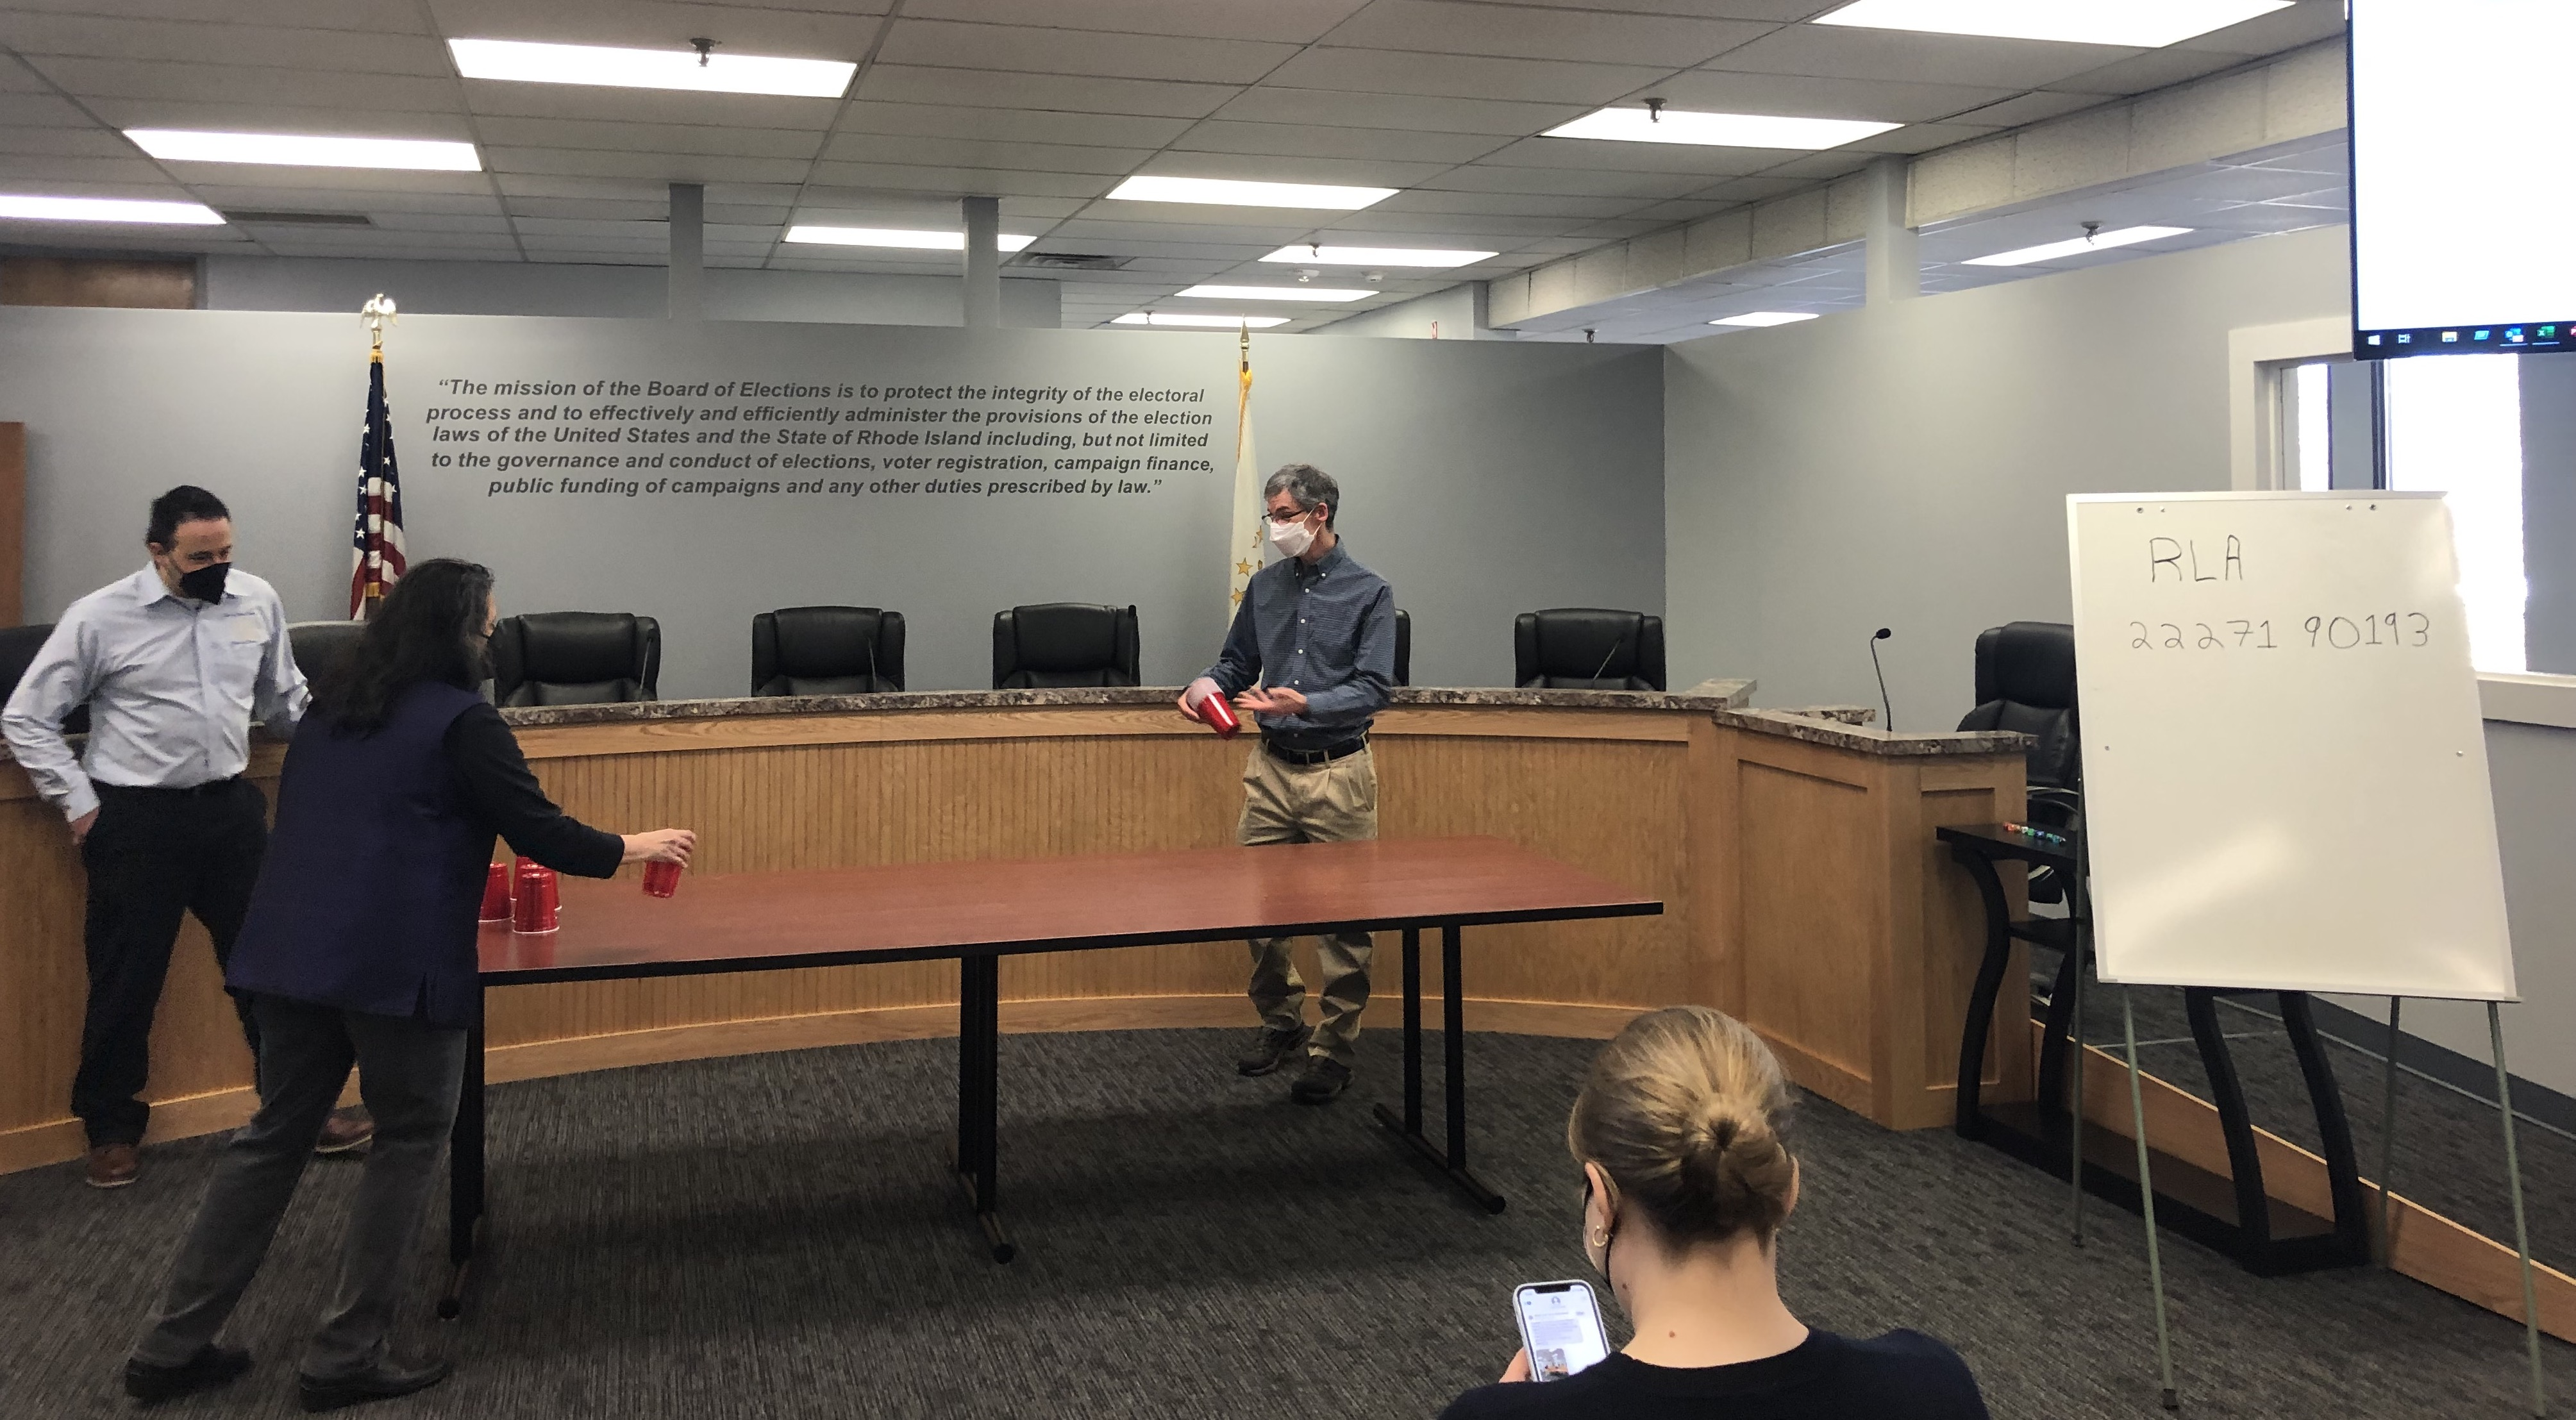
\includegraphics[width=1.0\textwidth]{dice.jpg}
\caption{
Professor Vora tosses her random-seed-generating 10-sided die, in a roll she dedicated to election officials everywhere.
The standing people from left to right are (1) Miguel Nunez, Rhode Island Deputy Director of Elections, 
(2) Professor Vora, and (3) Mark Lindeman, Verified Voting Director.
}
\end{figure}

\end{block}

\begin{block}{Simulations}

\begin{figure}[h]
\centering
\begin{minipage}{.49\textwidth}
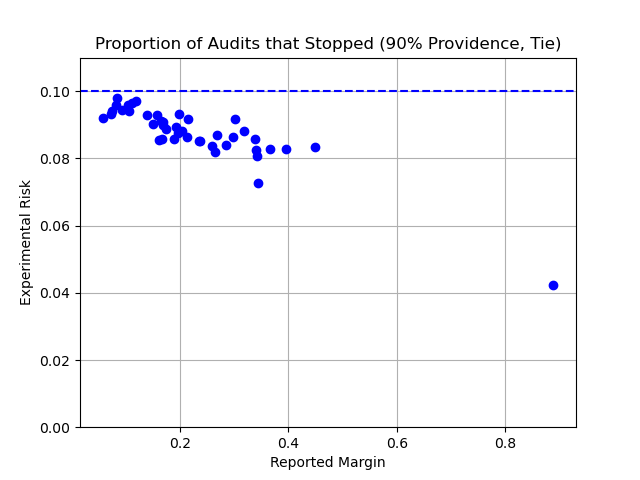
\includegraphics[width=\textwidth]{prov_risk.png}
\label{fig:bravo_risk}
\end{minipage}
\begin{minipage}{.49\textwidth}
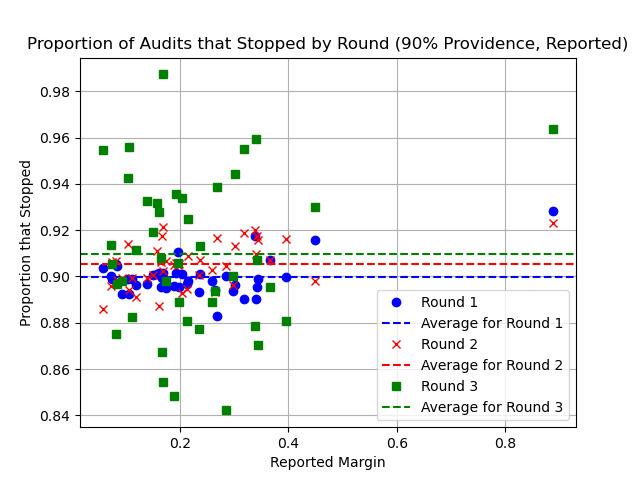
\includegraphics[width=1.0\textwidth]{prov_sprob.png}
\label{fig:minerva_risk}
\end{minipage}
\caption{
The left plot shows the fraction of \Prov audits that stopped in any of the $5$ rounds when the underlying election was a tie
where each round size is selected to achieve $\chi_j=0.9$.
The right plot shows the fraction of \Prov audits that stopped in any of the $5$ rounds when the underlying election was a tie for rounds
$j=1,2,3$ and $\chi_j=0.9$.
}
\label{fig:prov-risk-sprob}
\end{figure}


\begin{figure}
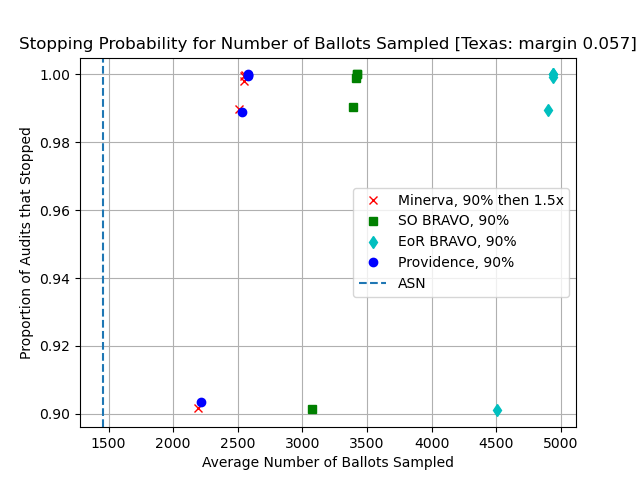
\includegraphics[width=.65\textwidth]{prov_asn.png}
\caption{Cumulative fraction of audits that stopped as a function of average number of sampled ballots for the state of Texas with margin $.057$ with first round stopping probability $\chi_1=0.9$. \Prov, \Minerva with multiplier $1.5$, and both implementations of \BRAVO are included.}
\end{figure}



\end{block}

\begin{block}{References}

%\footnotesize{
\bibliographystyle{plain}
\bibliography{audits}
%}

\end{block}

\end{column}

\separatorcolumn
\end{columns}
\end{frame}
\end{document}
